% ---------------------------------------------------------------------------------------------------------------
% TEMPLATE PARA TRABALHO ACADEMICOS
% Institudo Federal do Paraná - IFPR
% Customização da classe abnTeX2 (http://www.abntex.net.br/) para as normas da IFPR
%----------------------------------------------------------------------------------------------------------------
% Codificação: UTF-8
% LaTeX:  abnTeX2          
% ---------------------------------------------------------------------------------------------------------------


% CARREGA CLASSE PERSONALIZADA DA IFPR--------------------------------------------------------------------------
\documentclass[%twoside,                   % Impressão em frente e verso
    	        oneside,                   % Impressão apenas frentehttps://www.overleaf.com/project/601d9fdf130d22b45e6e96ff
]{configuracoes/ifpr-abntex2}


% INCLUI ARQUIVOS DE CONFIGURAÇÕES-------------------------------------------------------------------------------
\include{configuracoes/pacotes}
\include{configuracoes/configuracoes-pdf}


% INCLUI ARQUIVOS DO TRABALHO DE CONCLUSÃO DE CURSO (PRÉ-TEXTUAIS, TEXTUAIS, PÓS-TEXTUAIS)-----------------------

% INSERE CAPA E FOLHA DE ROSTO
% CAPA---------------------------------------------------------------------------------------------------

% ORIENTAÇÕES GERAIS-------------------------------------------------------------------------------------
% Caso algum dos campos não se aplique ao seu trabalho, como por exemplo,
% se não houve coorientador, apenas deixe vazio.
% Exemplos: 
% \coorientador{}
% \departamento{}

% DADOS DO TRABALHO--------------------------------------------------------------------------------------
\titulo{ TÍTULO }
\titleabstract{}
\autor{Nome comlete}
\autorcitacao{SOBRENOME, Nome} % Sobrenome em maiúsculo
\local{Cidade}
\data{2023}

% NATUREZA DO TRABALHO-----------------------------------------------------------------------------------
% Opções: 
% - Trabalho de Conclusão de Curso (se for Graduação)
% - Dissertação (se for Mestrado)
% - Tese (se for Doutorado)
% - Projeto de Qualificação (se for Mestrado ou Doutorado)
\projeto{Trabalho de Conclusão de Curso}

% TÍTULO ACADÊMICO---------------------------------------------------------------------------------------
% Opções:
% - Técnico em Informática
% - Bacharel ou Tecnólogo (Se a natureza for Trabalho de Conclusão de Curso)
% - Mestre (Se a natureza for Dissertação)
% - Doutor (Se a natureza for Tese)
% - Mestre ou Doutor (Se a natureza for Projeto de Qualificação)
\tituloAcademico{Técnico em Informática}

% ÁREA DE CONCENTRAÇÃO E LINHA DE PESQUISA---------------------------------------------------------------
% Se a natureza for Trabalho de Conclusão de Curso, deixe ambos os campos vazios
% Se for programa de Pós-graduação, indique a área de concentração e a linha de pesquisa
\areaconcentracao{Trabalho de Conclusão de Curso}
\linhapesquisa{}

% DADOS DA INSTITUIÇÃO-----------------------------------------------------------------------------------
% Se a natureza for Trabalho de Conclusão de Curso, coloque o nome do curso de graduação em "programa"
% Formato para o logo da Instituição: \logoinstituicao{<escala>}{<caminho/nome do arquivo>}
\programa{Nome do programa}
\departamento{Departamento}
\instituicaoS{Nome da Instituição associada se existir}
\instituicao{Nome da Instituição}
\logoinstituicao{0.101}{dados/figuras/Logo_IFPR} 

% DADOS DOS ORIENTADORES---------------------------------------------------------------------------------
%\orientador{Nome do coorientador}
\orientador[Orientadora:]{Nome do coorientador}
\instOrientador{IFPR}

%\coorientador{Nome do coorientador}
\coorientador[Coorientadora:]{Nome do coorientador}
\instCoorientador{IFPR}

% FOLHA DE ROSTO--------------------------------------------------------------------------------------------------------

% TRABALHO DE CONCLUSÃO DE CURSO
\preambulo{{\imprimirprojeto} apresentado ao {\imprimirprograma} da {\imprimirinstituicao}, como requisito parcial para a obtenção do título de {\imprimirtituloAcademico}.}

% DISSERTAÇÃO DE MESTRADO
%\preambulo{\large Dissertação de pesquisa apresentado no Conselho Acadêmico do Programa de Pós-Graduação em Sustentabilidade como parte integrante dos requisitos para a defesa de dissertação.}
%\preambulo{{\imprimirprojeto} apresentada ao Programa de \mbox{Pós-graduação} da {\imprimirinstituicao}, como requisito parcial para obtenção do título de {\imprimirtituloAcademico}.}

% TESE DE DOUTORADO
% \preambulo{{\imprimirprojeto} apresentada ao Programa de \mbox{Pós-graduação} da {\imprimirinstituicao}, como requisito parcial para a obtenção do título de {\imprimirtituloAcademico}.}

% PROJETO DE QUALIFICAÇÃO DE MESTRADO OU DOUTORADO
%\preambulo{{\imprimirprojeto} apresentado ao Programa de \mbox{Pós-graduação} da {\imprimirinstituicao}, como requisito parcial para a obtenção do título de {\imprimirtituloAcademico}.}

% OBSERVAÇÕES-----------------------------------------------------------------------------------------------------------
% Altere este arquivo APENAS comentando as linhas que não se aplicam ao tipo de trabalho acadêmico desejado.



\begin{document}

\pretextual
\imprimircapa                                               	           % Comando para imprimir Capa
\imprimirfolhaderosto{}                               		   % Comando para imprimir Folha de rosto
% INSERE ELEMENTOS PRÉ-TEXTUAIS

\begin{figure}[H]
   \includegraphics[width=1.1\linewidth]{dados/figuras/ficha catalografica Alex.pdf}
\end{figure}

\imprimirfolhadeaprovacao

% DEDICATÓRIA------------------------------------------------------------------

\renewcommand{\dedicatorianame}{DEDICATÓRIA}

\begin{dedicatoria}

Dedico esse trabalho ...

\end{dedicatoria}
          			   % Dedicatória
% AGRADECIMENTOS---------------------------------------------------------------

\begin{agradecimentos}[AGRADECIMENTOS]

Primeiramente agradeço a Deus, pela vida.

\end{agradecimentos}
        			   % Agradecimentos
% EPÍGRAFE---------------------------------------------------------------------

\renewcommand{\epigraphname}{EPÍGRAFE}

\begin{epigrafe}

\textit{A matemática, olhada corretamente, possui não apenas verdade, mas suprema beleza, uma beleza fria e austera, como aquela da escultura, sem apelo a qualquer parte da nossa natureza mais fraca, sem as encantadoras armadilhas da pintura ou da música, mas sublimemente pura, e capaz de uma rigorosa perfeição que somente a maior das artes pode exibir. (RUSSELL, Bertrans, 1970).}

\end{epigrafe}

% OBSERVAÇÕES------------------------------------------------------------------
% Altere o texto para inserir a epígrafe do seu trabalho

              			   % Epígrafe
% RESUMO--------------------------------------------------------------------------------

\begin{resumo}[RESUMO]
\begin{SingleSpacing}


Resumo 

\vspace{1cm}

\textbf{Palavras-chave}: Palavras-chave

\end{SingleSpacing}
\end{resumo}

% OBSERVAÇÕES---------------------------------------------------------------------------
% Altere o texto inserindo o Resumo do seu trabalho.
% Escolha de 3 a 5 palavras ou termos que descrevam bem o seu trabalho 

             			   % Resumo em Português
% ABSTRACT--------------------------------------------------------------------------------

\begin{resumo}[ABSTRACT]
\begin{SingleSpacing}


Abstract

\vspace{1cm}
		
\textbf{Keywords}: key words

\end{SingleSpacing}
\end{resumo}

% OBSERVAÇÕES---------------------------------------------------------------------------
% Altere o texto inserindo o Abstract do seu trabalho.
% Escolha de 3 a 5 palavras ou termos que descrevam bem o seu trabalho 
             		           % Resumo em Inglês
\include{estrutura/pre-textuais/listas/listas-ilustracoes/lista-figuras}   % Lista de Figuras
%% LISTA DE GRÁFICOS----------------------------------------------------------------

\renewcommand{\listofquadrosname}{LISTA DE GRÁFICOS}

\pdfbookmark[0]{\listofquadrosname}{loq}
\listofquadros*
\cleardoublepage

% OBSERVAÇÕES---------------------------------------------------------------------
% Este arquivo não necessita de ser editado. A lista é gerada automaticamente.
   % Lista de Quadros
\include{estrutura/pre-textuais/listas/lista-tabelas}         		   % Lista de Tabelas
% LISTA DE ABREVIATURAS E SIGLAS----------------------------------------------------------

\begin{siglas}
    \item[DSC] Calorimetria exploratória diferencial
    \item[ESL] Equilíbrio sólido-líquido
    \item[GA] Algoritmo Genérico
    \item[GRG] Gradiente Reduzido Generalizado
    \item[NRTL] \textit{Nonrandom Two Liquid Theory}
    \item[PIM] Programação Inteira Mista linear
    \item[PL] Programação Linear
    \item[PNL] Programação Não-linear
    \item[UNIQUAC] \textit{Quasi-chemical Theory}
\end{siglas}

% OBSERVAÇÕES-----------------------------------------------------------------------------
% Altere a lista acima para definir os acrônimos e siglas utilizados neste trabalho
          		   % Lista de Abreviaturas e Siglas
% LISTA DE SÍMBOLOS------------------------------------------------------------

\begin{simbolos}
    \item[$R$] Constante universal dos gases
    \item[$\Delta H_{f}$] Entalpia de fusão
    \item[$f$] Fugacidade
    \item[$G$] Energia livre de Gibbs
    \item[$NC$] Número de componentes
    \item[$NF$] Número de fases
    \item[$A_{ij}$ ou $A_{12}$] Parâmetro de Margules
    \item[$\mu$] Potencial químico
    \item[$P$] Pressão
    \item[$T$] Temperatura
    \item[$T_{f}$] Temperatura de Fusão
    \item[$U$] Energia interna
    \item[$V$] Volume
    \item[$\underline{V}$] Volume molar
\end{simbolos}

% OBSERVAÇÕES-------------------------------------------------------------------
% Altere a lista acima para definir os símbolos utilizados no trabalho
        		   % Lista de Símbolos
%\include{estrutura/pre-textuais/listas/listas-diversas/lista-algoritmos}   % Lista de Algoritmos
\include{estrutura/pre-textuais/sumario}               			   % Sumário

\textual
% INSERE ELEMENTOS TEXTUAIS
% INTRODUÇÃO-------------------------------------------------------------------

\chapter{INTRODUÇÃO}
\label{chap:introducao}

\lipsum[1-2]\cite{Iezzi_fund1}

\lipsum[3-4]\cite{Leggieri2018a, Muller2019}

\begin{citacao}
	 Segundo \cite{AnaF} \lipsum[5-5] 
\end{citacao}

%Introdução
%OBJETIVOS--------------------------------------------------------

\chapter{OBJETIVOS}
\label{chap:objetivos}

\section{Objetivo Geral}



\section{Objetivo Específico}

%Objetivos
% JUSTIFICATIVA------------------------------------------------------------------

\chapter{JUSTIFICATIVA}
\label{chap:justifiativa}

Um dos pontos importantes é escolha das matérias-primas utilizadas na fabricação do biodiesel, as quais influenciam as propriedades do mesmo, segundo Dias (\citeyear{Angelica})

O combustível é mais vulnerável à oxidação;  tem pior capacidade de armazenamento,  menos fluidez no clima frio e menor estabilidade da oxidação. Estas características tornam mais difícil comercializar o biodiesel obtido de gorduras animais, que são mais insaturadas.  \cite{Leggieri2018a}

\cite{DeMarco2019,Prausnitz,Goulart2019}

\cite{Rocha2011,Leggieri2018a,Costa2007,Wei2009,Boudouh2016,Costa2012,Costa2009}

%Justificativa
% REVISÃO BIBLIOGRÁFICA------------------------------------------------------------------

\chapter{REVISÃO DE LITERATURA}
\label{chap:revisao_bibliografica}
\section{Objetivos de desenvolvimento sustentável}

Atualmente, petróleo bruto, carvão e gás, que são fosseis e não renováveis, ainda são dominantes na produção de combustíveis. A utilização dos combustíveis fosseis gera diversos impactos ambientais não desejáveis como: a poluição do ar e o aquecimento global \cite{Gebremariam2018}.

\section{Álcoois e Ácidos  carboxílicos}

\begin{citacao}
	Eles possibilitam uma variedade de texturas. Nos  fármacos desempenha um papel importante nas propriedades  ponto de fusão e solubilidade, caracterizadas pelo equilíbrio de fase sólido-líquido. \cite{Barbosa2012}
\end{citacao}

Eles possibilitam uma variedade de texturas. Nos  fármacos desempenha um papel importante nas propriedades  ponto de fusão e solubilidade, caracterizadas pelo equilíbrio de fase sólido-líquido. \cite{Barbosa2012}

O biodiesel é produzido por meio da transesterificação,  reação na qual  os triglicerídeos reagem com álcoois, na presença de um catalisador, para produzir esteres de  ácido graxo e glicerina, essa produzida como subproduto \cite{Hoekman2012}.

\begin{table}[H]
    \centering
    \caption{Grupos de ácidos graxos típicos em biodiesel}
    \begin{tabular}{lccc}
    \hline
    Nome & N$^0$ CAS  & Fórmula Molecular  & Estrutura Molecular  \\
    \hline
    Ácido Láurico & 143-07-7 & \ch{C12H24O2} & \raisebox{-0.5\height}{\includegraphics[width=0.4\linewidth]{dados/figuras/Ac_laurico.png}} \\
    Ácido Miristico & 544-63-8 & \ch{C14H28O2} & 
    \end{tabular}
    \label{tab:Grupo}
\end{table}

Consequentemente,  suscetíveis à erosão e ocorrência de deficiência de macro e micronutrientes \cite{Fonseca2005}.
    
A região  Noroeste do Paraná produz dentre outras culturas: \textit{Glycine max} (soja), \textit{Ricinus communis} (mamona) e \textit{Crambe abyssinica} (crambe), potenciais matérias-primas para o aumento da produção de biodiesel. A Tabela \ref{tab:angelica} observa-se a composição de ácidos graxos nesses óleos em percentagem \cite{Angelica}.

\begin{table}[H]
\centering
\caption{Composição dos ácidos graxos do óleo de soja, de rícino e de cambre.}
\begin{tabular}{lp{2.5cm}p{2.5cm}p{2.5cm}}
\hline
\multirow{2}{*}{Nomenclatura do Ácido} & \multicolumn{3}{l}{Porcentagem de ácidos carboxílicos totais (\%)}  \\
    & Soja  & Rícino & Crambe  \\
    \hline
     Ácido Láurico      & 0,1 (máx.)  &  & \\
     Ácido Mirístico    & 0,2 (máx.)  &  &  \\
     Ácido Palmítico    & 9,9 - 12,2  & 0,9 -1,5 & 3,4  \\
     Ácido Palmitoléico & Traços -0,2 &  &  \\
     Ácido Esteárico    & 3 - 5,4     & 1,4-2,1  & 1,1 \\
     Ácido Oleico       & 17,7 - 26   & 3,1-5,9 & 17,8 \\
     Ácido Linoléico    & 49,7 - 56,9 & 2,9- 6,5 & 6,1 \\
     Ácido Linolênico   & 5,5 - 9,5   &  & 2,8 \\
     Ácido Araquídico   & 0,2 - 0,5   &  & 1,7 \\
     Ácido Gadolêico    & 0,1 - 0,3   &  &  \\
     Ácido Behênico     & 0,3 - 0,7   &  & 3,7 \\
     Ácido Erúcico      & 0,3 (máx.)  &  & 56,7 \\
     Ácido Lignocérico  & 0,4 (máx.)  &  &  \\
     Ácido Eicosenóico  &             &  & 6,7 \\
     Ácido Ricinoléico  &             & 84,0 -91,0 &  \\
     \hline
\end{tabular}
\label{tab:angelica}
\end{table}

\section{Equilíbrio de fases sólido-líquido}
	
Para que não ocorra ambiguidades o número de propriedades intensivas do estado de equilíbrio é definido pela \textit{regra de fases de Gibbs}. \cite{Prausnitz}
	
	%Número de propriedades intensivas = número de componentes - número de fases +2

	\begin{description}
		\item[i)] número de mol deve ser um valor positivo:
		\begin{equation}
		\eta_{ij}\geqslant 0,\  \ i=1,2,\ldots,NC \mbox{ e } j=1,2,\ldots,NF
		\end{equation}
		\item[ii)] conservação de massa sem reações químicas:
		\begin{equation}
		\sum_{i=1}^{NC}\eta_{ij}=\eta_{i},\  \ i=1,2,\ldots,NC
		\end{equation}
	\end{description}
	em que $\eta_{i}$ é número total de mols do componente $i$.
	\cite{Sandlel,Barbosa2012,Prausnitz}
	
	\section{Cálculo do equilíbrio para substância pura}
	
	\hspace{5mm} O coeficiente de atividade para a fase líquida é definida para o estado padrão da substância líquida pura sub-resfriada na temperatura $T$ sobre uma pressão é representada pela equação:
	\begin{equation}\label{eq:atividade_1}x_i=\frac{f_{i(\mbox{\tiny sólido puro})}}{\gamma_{i}f_{i(\mbox{\tiny líquido sub-resfriado puro})}}
	\end{equation}
	para simplificar a notação
	\begin{equation*}
	f_{i}^{S}=f_{i(\mbox{\tiny sólido puro})}
	\end{equation*}
	e
	\begin{equation*}
	f_{i}^{L}=f_{i(\mbox{\tiny líquido sub-resfriado puro})}
	\end{equation*}
	em que as duas fugacidade depende apenas das propriedades da substância relacionada a componente $i$ e são independentes da natureza da substância. %A razão entre essas duas fugacidades.
	

	\subsection{Ácido Mirístico}
	\label{sec:1}
	\begin{itemize}
		\item Estrutura
		\begin{figure}[H]
			\centering
			\includegraphics[width=0.7\linewidth]{dados/figuras/Ac_miristico.png}
			\caption[Ácido Mirístico]{Ácido Mirístico  NIST \textit{National Institute of Standards and Technology}}
			\label{fig:nist1}
		\end{figure}
		\item Número do CAS: 544-63-8
		\item Fórmula Molecular: \ch{C14H28O2}
		\item Temperatura de fusão ($T_f$)=327.55 k
		\item Entalpia ($\Delta H_{f}$)=10.771955 kcal/mol
	\end{itemize}
	
	\subsection{Ácido Esteárico}
	\label{sec:2}
	\begin{itemize}
		\item Estrutura
		\begin{figure}[H]
			\centering
			\includegraphics[width=0.7\linewidth]{dados/figuras/Ac_estearico.png}
			\caption[Ácido Esteárico]{Ácido Esteárico NIST \textit{National Institute of Standards and Technology}}
			\label{fig:nist2}
		\end{figure}
		\item Número do CAS: 57-11-4
		\item Fórmula Molecular: \ch{C18H36O2}
		\item Temperatura de fusão ($T_f$)=342.75 k
		\item Entalpia ($\Delta H_{f}$)=14.64126 kcal/mol
	\end{itemize}
	
	\subsection{Ácido Palmítico}
	\label{sec:3}
	\begin{itemize}
		\item Estrutura
		\begin{figure}[H]
			\centering
			\includegraphics[width=0.65\linewidth]{dados/figuras/Ac_palmitico.png}
			\caption[Ácido Palmítico]{Ácido Palmítico NIST \textit{National Institute of Standards and Technology}}
			\label{fig:nist3}
		\end{figure}
		\item Número do CAS: 57-10-3
		\item Fórmula Molecular: \ch{C16H32O2}
		\item Temperatura de fusão ($T_f$)=336.00 k
		\item Entalpia ($\Delta H_{f}$)=80.252256 kcal/mol
	\end{itemize}
	
	\subsection{1-Hexadecanol}
	\label{sec:4}
	\begin{itemize}
		\item Estrutura
		\begin{figure}[H]
			\centering
			\includegraphics[width=0.8\linewidth]{dados/figuras/Hexadecanol.png}
			\caption[1-Hexadecanol]{1-Hexadecanol NIST \textit{National Institute of Standards and Technology}}
			\label{fig:8}
		\end{figure}
		\item Número do CAS: 36653-82-4
		\item Fórmula Molecular:\ch{C16H34O}
		\item Temperatura de fusão ($T_f$)=322,35k
		\item Entalpia ($\Delta H_{f}$)=8.025226 kcal/mol
	\end{itemize}
	


		%RevisãoBibliográfica
% MODELAGEM MATEMÁTICA PARA A OTIMIZAÇÃO DO EQUILÍBRIO SÓLIDO-LÍQUIDO------------------------------------------------------------------

\chapter{MODELAGEM MATEMÁTICA}
\label{chap:modelagem_matematica}

\section{Otimização}

O conceito de \textit{otimização} é uma forma de trazer uma solução satisfatória para problemas complexos que exigem a tomada de decisão ou alocação. \cite{Luenberger2016}

\section{Programação Não Linear}

Problemas reais são na grande maioria formulados por restrições, como a política de produção em uma grande empresa ou planejamento da agência governamental, são problemas de programação não linear com restrições.

Em geral o problema de programação é indicada por:
\begin{equation}
\begin{array}{rcccc}
\mbox{minimização} & f(x) & & & \\
\mbox{sujeita as condições} & h_{i}(x)&=&a_{i}, & i=1,2,\ldots,m \\
& g_ {j}(x)&\leq&b_j, & j=1,2,\ldots,p\\
& x\in S & & & \\
\end{array}
\end{equation}

Em que $x$ é um vetor n-dimensional $x=(x_{1},x_{2},\ldots,x_{n})$, $f_{i}$ e $h_i$ são funções reais das variáveis $x_{1},x_{2},\ldots,x_{n}$. A função $f$ é a \textit{função objetivo}, $g$, $h$ e o conjunto $S$ são as restrições do problema; com os parâmetros $a_i$ e $b_j$. \cite{Luenberger2016, Rocha2009a}

\section{Convexidade}

Os conceitos relacionados aos conjuntos \textit{convexos} são relevantes teoria da otimização, representada pela Figura \ref{fig:convexSet} na forma bidimensional, que por sua vez é essencial para um estudante de otimização ter conhecimento de suas propriedades mais fundamentais. \cite{Luenberger2016, Rocha2009a}

\begin{definicao}
	Dado um conjunto $C\subset E^{n}$ diz que é \textbf{convexo} se para qualquer $x_{1}, x_{2} \in C$ e para todo $\alpha\in\mathbb{R}$, tal que o ponto $\alpha x_{1}+(1-\alpha)x_{2}\in C$.
\end{definicao}

%\begin{comment}
\begin{figure}[H]
	\centering
	\subbottom[Convexo]{
		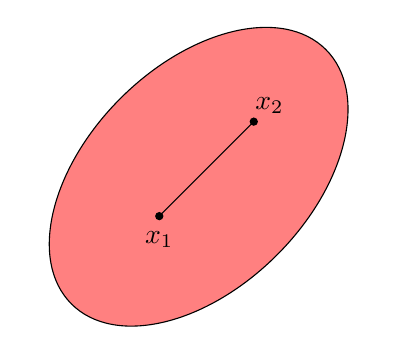
\begin{tikzpicture}
		\draw[rotate=-45,fill=red!50] (0,0) ellipse (40pt and 65pt);
		\draw (-0.5,-0.5) -- (0.7,0.7);
		\fill (-0.5,-0.5) circle[radius=1.5pt];
		\fill (0.7,0.7) circle[radius=1.5pt];
		\node at (-0.5,-0.8) {$x_1$};
		\node at (0.9,0.9) {$x_2$};
		\end{tikzpicture}}
	\hspace{2cm}
	\subbottom[Não Convexo]{
		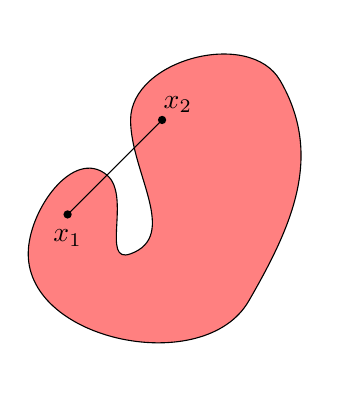
\begin{tikzpicture}
		\draw[fill=red!50] (0,0) to [out=140,in=90] (-1,-1)
		to [out=-90,in=240] (1.8,-1.6)
		to [out=60,in=-60] (2.2,1.2)
		to [out=120,in=90] (0.3,0.7)
		to [out=-90,in=20] (0.3,-1)
		to [out=200,in=-40] (0,0);
		\draw (-0.5,-0.5) -- (0.7,0.7);
		\fill (-0.5,-0.5) circle[radius=1.5pt];
		\fill (0.7,0.7) circle[radius=1.5pt];
		\node at (-0.5,-0.8) {$x_1$};
		\node at (0.9,0.9) {$x_2$};
		\end{tikzpicture}}
	\caption{Convexidade de conjuntos}
	\label{fig:convexSet}
\end{figure}

\section{\textit{Softwares} Utilizados}

Os \textit{softwares} utilizados para o desenvolvimento do trabalho, foram descritos nos subitens que seguem.

\subsection{\textit{Geogebra}}
Para a coleta de pares ordenados e organização das misturas binárias para fins de cálculos vamos utilizar o \textit{software} \textit{Geogebra}\footnote{Site do Geogebra \url{https://www.geogebra.org/}} é um \textit{software} de código aberto Figura \ref{fig:11}, oferecido para várias plataformas, com a finalidade didática e de pesquisa. 
\begin{figure}[H]
	\centering
	\includegraphics[width=0.9\linewidth 
	%,height=0.4\textheight
	]{dados/figuras/Geogebra_1.png}
	\caption[Site do Geogebra]{Site do Geogebra}
	\label{fig:11}
\end{figure}


\subsection{\textit{PyCharm} e \textit{R}}

Os \textit{software} \textit{PyCharm}\footnote{Site do \textit{PyCharm} \url{https://www.jetbrains.com/pt-br/pycharm/}} (FIGURA \ref{fig:11}) possui licença gratuita com restrições, disponíveis para as principais plataformas e, conjuntamente com a utilização da biblioteca \textit{R}\footnote{A base de dados para implementação de modelos estatísticos disponível no site \url{https://cran.r-project.org/}} (FIGURA \ref{fig:11}), se apresentam como uma base para implementação de algoritmos e modelos estatísticos. 



\subsection{Editor de texto \LaTeXe}

\LaTeXe  é o \textit{software} de código aberto de alta qualidade afim de produzir impressões profissionais e arquivos PDF, cuja base de dados \textit{TexLive}\footnote{Se encontra no site \url{http://tug.org/texlive/}} para plataformas Linux e macOS, organizada por \textit{TeX User Group} instituição sem fins lucrativos fundada em 1980, composto por \TeX\ \ criado por Donald Knuth e a mais conhecida ou difundida \textit{MikTex}\footnote{Se encontra no site \url{https://miktex.org/}} para todas as plataforma. A interface gráfica foi utilizado o \textit{TeXstudio}\footnote{Se encontra no site \url{https://www.texstudio.org/}} e \textit{Overleaf}\footnote{Se encontra no site \url{https://pt.sharelatex.com/}} uma ferramenta online para trabalhos colaborativos com o sistema de versionamento podendo ver quais são as modificações feitas por cada um colaborador. A a principal finalidade do \LaTeX é trazer uma tipografia de alta qualidade com o intuito trazer uma leitura mais agradável visualmente, com a biblioteca \textit{amsmath} para escrever fórmulas matemática, \textit{tikz} para criar desenhos vetoriais como os desenhos Figura\ref{fig:convexSet} e Figura\ref{fig:11}, \textit{chemformula} para fórmulas químicas, colabora com citação, facilita indexação de elementos e entre outras funcionalidades. \cite{latexchemformula,latexabntex2,latextikz,tex}


%Modelagerm_Matemática
\chapter{MATERIAIS E MÉTODOS}
\label{Material_metodo}

\section{Materiais}
\hspace{0.5cm} \lipsum[13-15]

\section{Métodos}

\hspace{0.5cm} \lipsum[13-15] \cite{Rocha2009a,Costa2007}

Segundo ROCHA \citeyear{Rocha2009a},\lipsum[13-15]

 %Materiais_métodos
\chapter{RESULTADOS E DISCUSSÕES}\label{chap:resultados}

A escala de cada diagrama de fase das misturas binárias são distintas, pelo fato de que cada ácido graxo ou álcool possui ponto de fusão distintos como podemos verificar nas seções \ref{sec:1} até \ref{sec:4}.

\section{Estudos de casos.}

\subsection{Sistema 1: Ácido Mirístico e Ácido Esteárico}\label{sistema1}

Na Figura \ref{fig:11} o diagrama de fase foi determinado pelos modelos termodinâmicos \textit{MA}, \textit{MS} e \textit{Wilson} implementado no \textit{GAMS} e o gráfico gerado pelo \textit{PyCharm} com biblioteca do \textit{R}. Os dados experimentais comparativos foram obtidos por COSTA 2009 por experimentos com o método de DSC.
\begin{figure}[H]
	\centering
	\includegraphics[width=1.06\linewidth 
	%,height=0.4\textheight
	]{dados/figuras/Miristico_estearico.png}
	\caption[Diagrama do equilíbrio sólido-líquido para mistura Ácido Mirístico e Ácido Esteárico]{Diagrama do equilíbrio sólido-líquido para mistura Ácido Mirístico(1) e Ácido Esteárico(2) (\textit{PyCharm}/$R$)}
	\label{fig:3}
\end{figure}

\section{Coeficiente de Determinação}

A propriedade do coeficiente de determinação é que:
\begin{itemize}
    \item $R^2\in [0;1]$
    \item $R^2=1$, $VD$ é explicada pela variação de $VI$ em 100\%
    \item $R^2=0$, $VI$ não tem influencia sobre $VD$.
\end{itemize}

O valor do $R^2$ é calculado pela fórmula
\begin{equation}
    R^2=\frac{\left(\displaystyle\sum_{i=1}^{n}x_i\cdot y_i-n\cdot\overline{x}\cdot\overline{y}\right)^2}{\left(\displaystyle\sum_{i=1}^{n}x_i^2-n\cdot\overline{x}^2\right)\times\left(\displaystyle\sum_{i=1}^{n}y_i^2-n\cdot\overline{y}^2\right)}
\end{equation}
em que $n$ quantidade de elementos da variável $VD$ ou $VI$, $x_i\in VI$ e $y_i\in VD$.
\begin{equation}
    \overline{x}=\frac{\displaystyle\sum_{i=1}^{n}x_i}{n}
\end{equation}
e
\begin{equation}
    \overline{y}=\frac{\displaystyle\sum_{i=1}^{n}y_i}{n}
\end{equation}

%\begin{center}
    %Coeficiente de determinação da variável dependente  técnicas de %DSC e variáveis independentes MA, MS ou Wilson
%\end{center}
\begin{table}[H]
    \caption{Coeficiente de Determinação}
    \centering
    \begin{tabular}{l|p{3cm}p{3cm}p{3cm}}
    %\multicolumn{4}{c}{\textbf{Coeficiente de determinação da variável dependente  técnicas de DSC e variáveis}}  \\ 
    %\multicolumn{4}{c}{\textbf{independentes MA, MS ou Wilson}} \\ 
    \hline
         & $R^2$ MA & $R^2$ MS & $R^2$ Wilson \\
    \hline
    Ac. Mirístico e Ac. Esteárico  & 0.9756  & 0.9706 & 0.9708 \\
    Ac. Palmítico e Ac. Esteárico  & 0.9699  & 0.8005 & 0.7040 \\
    %Ac. Palmítico e Ac. Esteárico  & 0.4955  & 0.5355 & 0.5057 \\
    Hexadecanol e Ac. Mirístico  & 0.2427  & 0.2328 & 0.2133 \\
    Hexadecanol e Tetradecanol  & 0.9804  & 0.9310 & 0.9887 \\
    Ac. Esteárico e Ac. Linoleico  & 0.1483  & 0.5592 & 0.8745 \\
    Ac. Palmítico e Ac. Linoleico  & 0.7490  & 0.5602 & 0.0000 \\
    \end{tabular}
    \label{tab:1}
\end{table}

 %Resultados
% CONCLUSÃO--------------------------------------------------------------------

\chapter{CONSIDERAÇÕES FINAIS}
\label{chap:conclusao}


\chapter{TRABALHOS FUTUROS}
\label{sec:trabalhosFuturos}

%Conclusão

\postextual
% INSERE ELEMENTOS PÓS-TEXTUAIS
\include{estrutura/pos-textuais/referencias}           			   % Referências
%\include{estrutura/pos-textuais/apendices}             			   % Apêndices
% ANEXO------------------------------------------------------------------------

\begin{anexosenv}
\partanexos

% Primeiro anexo---------------------------------------------------------------
\chapter{Banco de dados e algoritmo}     % edite para alterar o título deste anexo
\label{chap:anexoA}

Os valores dos pares ordenados com as misturas binárias, temperaturas, algoritmos da construção dos diagramas e do coeficientes de determinação em $R$, se encontram no repositório do \textit{GitHub}. Um sistema de versionamento e armazenamento de dados.

\url{https://github.com/alexissamumoriya/Algoritmo_Diagramas_compartilhados}

\end{anexosenv}
               			   % Anexos

\end{document}
